\documentclass[aspectratio=169]{beamer}
\usepackage{fontspec}
\usepackage{hyperref}
\usepackage{ccicons}
\protrudechars=2 % or \pdfprotrudechars=2 and
\adjustspacing=2 %    \pdfadjustspacing=2 with luatex < v0.85
\usepackage{amsmath}
\usepackage{graphicx}
\usepackage[table]{xcolor} % Για χρωματισμούς στις γραμμές και τις στήλες
\usepackage{xcolor}
\usepackage{polyglossia}
\usepackage{csquotes}
\usepackage[symbol]{footmisc}
\setmainlanguage{greek}
\setotherlanguage{english}
\setmainfont[Numbers={OldStyle, Proportional},
Ligatures=TeX]{Linux Libertine O}
\newfontfamily\greekfont{Linux Libertine O}
\newfontfamily\englishfont{Linux Libertine O}
\newfontfamily\greekfontsf{Linux Libertine O}
\usetheme{Madrid}
\usecolortheme{beaver}
\title{Εισαγωγή στο λογισμικό της διαδικτυακής αναμετάδοσης}
\subtitle{OBS (Open Broadcaster Software) και πλατφόρμες διαδικτυακής αναμετάδοσης} 
\author{Ερμής Δούλος (\textit{dit17046@uop.gr})}
\begin{document}

\begin{frame}
  \titlepage
  \begin{center}
    % GitHub Link
    \href{https://github.com/doblador42}{\textbf{Github Profile:}}\\
    % QR Code
    
\includegraphics[width=0.13\textwidth]{images/qrcode.png}
  \end{center}
\end{frame}


\begin{frame}{Επισκόπηση}
  \begin{block}{Περιεχόμενα}
\begin{itemize}
\item Ανασκόπηση του λογισμικού μιας τηλεμετάδοσης
\item Εισαγωγή στο OBS
\begin{itemize}
  \item Εγκατάσταση
  \item Ρύθμιση
  \item Χρήση
        \begin{itemize}
          \item Πηγές
          \item Σκηνές
          \item Επιλογές διάταξης
        \end{itemize}
\end{itemize}
\item Πλατφόρμες αναμετάδοσης
\begin{itemize}
  \item YouTube
  \item Zoom
  \item Webex
  \item Teams
\end{itemize}
\item Παραδείγματα
\end{itemize}
\end{block}
\end{frame}
\begin{frame}{Διάγραμμα όλης της αναμετάδοσης}
  \begin{center}
    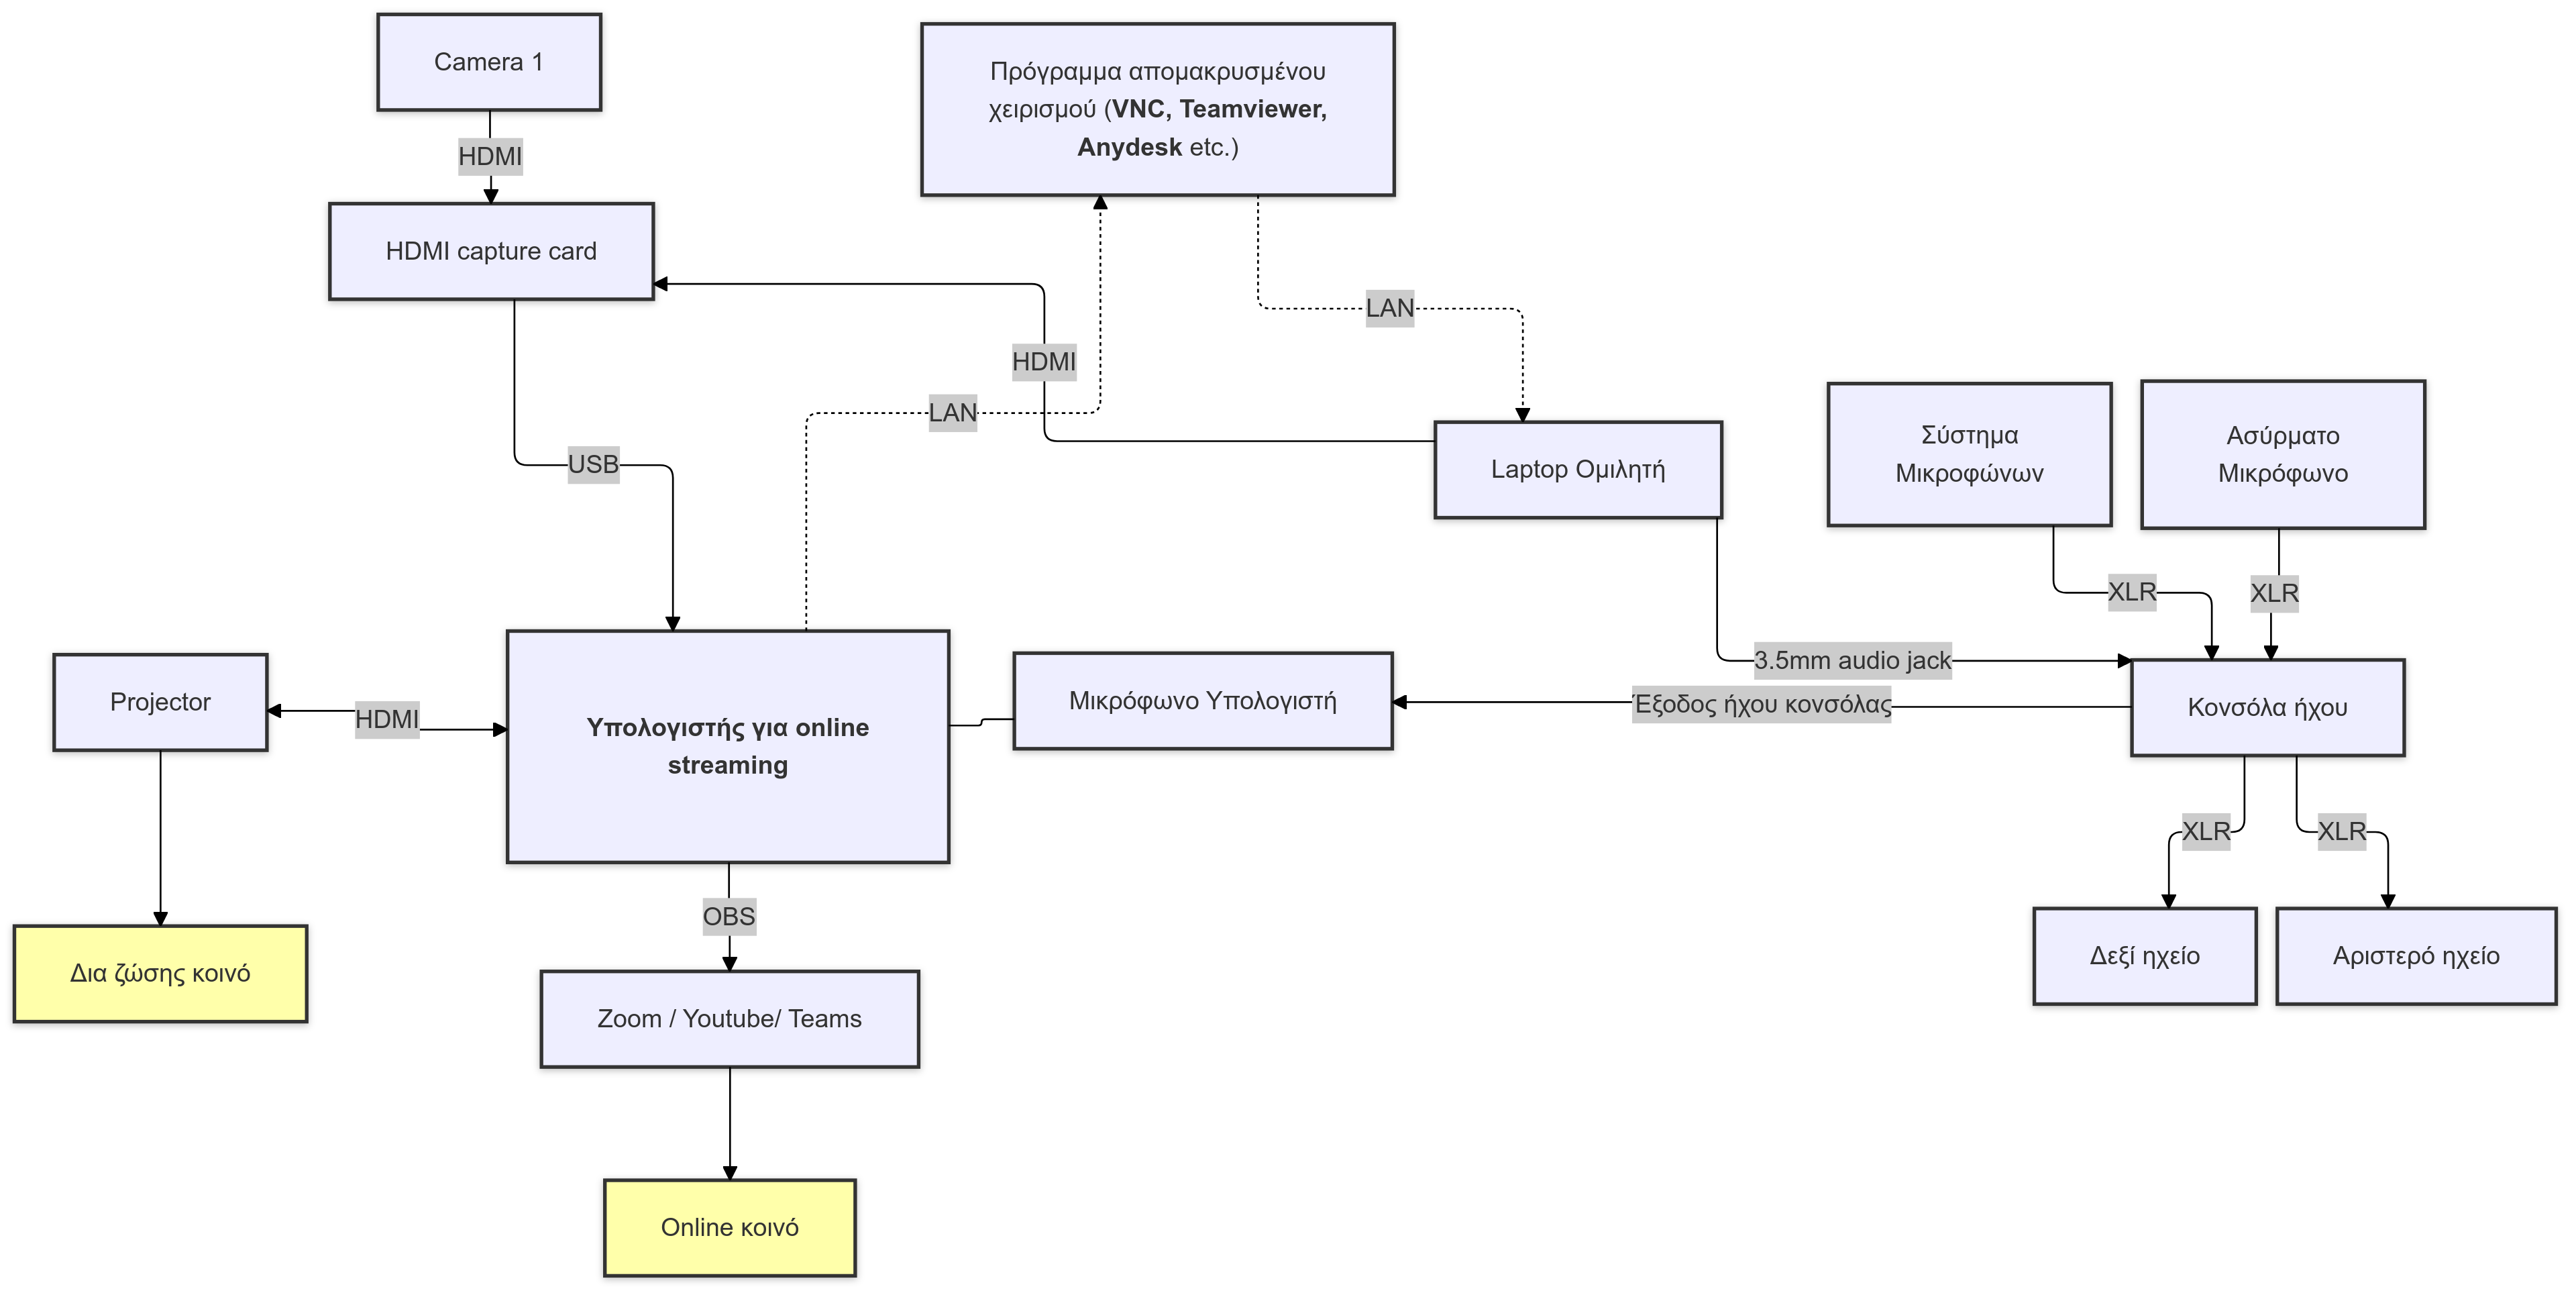
\includegraphics[width=0.9\textwidth]{images/diagram.png}
  \end{center}
\end{frame}
\begin{frame}{Τι χρειαζόμαστε σε λογισμικό για μια διαδικτυακή αναμετάδοση;}
  \begin{block}{Πρόγραμμα αναμετάδοσης}
    \begin{itemize}
      \item Εύκολη χρήση\footnote{Χωρίς πολλές πολύπλοκες ρυθμίσεις και προσβάσιμο και σε μη ειδικούς της πληροφορικής}
      \item Ευελιξία\footnote{Δυνατότητα προσθήκης πολλαπλών πηγών και παραμετροποίησης της εμφάνισης τους}
      \item Επαγγελματική ποιότητα\footnote{Καλή ποιότητα εικόνας και ήχου χωρίς διαλείψεις και εκπλήξεις}
      \item Ελεύθερο λογισμικό\footnote{Διότι είναι δωρεάν και ανοιχτού κώδικα}
    \end{itemize}
  \end{block}
\end{frame}

\begin{frame}{Άδεια Χρήσης}
  \begin{center}
    \ccbysa
  \end{center}
  \begin{center}
    Άδεια \href{https://creativecommons.org/licenses/by/4.0/}{Creative Commons Αναφορά Δημιουργού 4.0 Διεθνές (CC BY 4.0)}.  Το παρόν διατίθεται υπό την
    \ccbysa
  \end{center}
  \begin{exampleblock}{Επιτρέπεται στον αποδέκτη:}
    \begin{itemize}
      \item Να μοιραστεί το έργο με άλλους.
      \item Να τροποποιήσει το έργο για προσωπική ή εμπορική χρήση.
      \item Να χρησιμοποιήσει το έργο σε παρουσιάσεις ή δημοσιεύσεις.
      \item Να αναφέρει τον δημιουργό του έργου όταν το χρησιμοποιεί.

    \end{itemize}
  \end{exampleblock}
\end{frame}
\end{document}
